\documentclass[11pt,a4paper]{article}
\usepackage[utf8]{inputenc}
\usepackage[T1]{fontenc}
\usepackage{lmodern}
\usepackage[margin=2.2cm]{geometry}
\usepackage{graphicx}
\usepackage{booktabs}
\usepackage{longtable}
\usepackage{array}
\newcolumntype{L}[1]{>{\raggedright\arraybackslash}p{#1}}
\usepackage{float}
\usepackage{xcolor}
\usepackage{amsmath}
\usepackage{caption}
\usepackage{enumitem}
\usepackage[hidelinks]{hyperref}
\graphicspath{{../../figures/}}

\definecolor{navy}{HTML}{1B2A4A}
\newcommand{\var}[1]{\texttt{\detokenize{#1}}}
\newenvironment{reading}{\par\smallskip\noindent\textbf{\color{navy}Interpretation.}\ }{\par\medskip}
\setlist{itemsep=2pt,topsep=3pt}
\captionsetup{font=small,labelfont=bf}
\widowpenalty=10000 \clubpenalty=10000
\setlength{\parskip}{4pt}\setlength{\parindent}{0pt}

\title{\textbf{Cross-Network Intrusion Analysis}\\[4pt]
\large Phase 5 --- Feature Engineering of the merged NetFlow data}
\author{Ahmed Hamouda}
\date{Notebook \texttt{08\_features\_netflow.ipynb}}

\begin{document}
\maketitle

\section{Goal and method}

\textbf{Requirement.} Explain feature selection, extraction / creation, encoding, and scaling / transformation when
appropriate, and justify the final feature set.

\textbf{Data.} The merged NetFlow table of phase 3: 17,551,848 behaviours from four networks (UNSW-NB15,
CSE-CIC-IDS2018, ToN-IoT, BoT-IoT). Every choice below is based on a decision of phase 2 or a finding of phase 4.

\textbf{Steps.} (0) starting columns; (1) creation of new features; (2) encoding of the code columns; (3) log
transformation and robust scaling; (4) feature selection; (5) final feature set; (6) PCA; (7) techniques not used.

\textbf{No train/test split.} The project stops before modelling. The steps that learn a value from the data (scaling, the
list of frequent application protocols, the selection) are fitted on all the data. \emph{In a modelling phase, these
steps must be refitted on the training part only, to avoid data leakage.}

\textbf{Sample.} Correlation, mutual information and PCA use one sample of up to 5,000 random behaviours from each
network $\times$ family group (102,058 rows), so every family counts. All other steps use all 17.5 million rows.

\section{Starting columns}

Nine columns are left out because they must never be features (phase 2 decisions):

\begin{table}[H]\centering\small
\caption{Columns left out before feature engineering.}
\begin{tabular}{p{8.4cm}p{6.4cm}}
\toprule
Columns & Reason \\
\midrule
\var{FLOW_START_MILLISECONDS}, \var{FLOW_END_MILLISECONDS} & reveal the lab's attack schedule (M2) \\
\var{L4_SRC_PORT}, \var{DNS_QUERY_ID} & random numbers chosen by the machine (M5) \\
\var{MIN_TTL}, \var{MAX_TTL}, \var{FTP_COMMAND_RET_CODE} & identify the lab's machines (M4, M10) \\
\var{Attack}, \var{network_type} & the raw label and the network name \\
\bottomrule
\end{tabular}
\end{table}

The starting point is \textbf{31 numeric traffic columns} (bytes, packets, durations, packet sizes, gaps between
packets, throughput, retransmissions) and \textbf{8 code columns} (destination port, protocol, application protocol and
its sub-code, client and server TCP flags, ICMP type, DNS query type). The labels (\var{attack_family},
\var{attack_label}, \var{is_attack}) and \var{count}, \var{source_dataset} are kept aside, never as features.

\section{Creation / extraction}

\begin{table}[H]\centering\footnotesize\setlength{\tabcolsep}{4pt}
\caption{New features, computed row by row.}
\begin{tabular}{p{3.0cm}p{5.6cm}p{6.4cm}}
\toprule
Feature & Formula & Why (phase 4 finding) \\
\midrule
\var{in_bytes_per_pkt} & \var{IN_BYTES} / \var{IN_PKTS} & size of the packets sent (probe vs transfer) \\
\var{out_bytes_per_pkt} & \var{OUT_BYTES} / \var{OUT_PKTS} (0 if no answer) & size of the packets received \\
\var{out_in_ratio} & \var{OUT_BYTES} / \var{IN_BYTES} & one-way traffic vs a conversation \\
\var{bytes_per_sec} & bytes (both ways) / duration & speed: floods are fast, slow attacks slow \\
\var{pkts_per_sec} & packets (both ways) / duration & packet rate \\
\var{no_answer} & \var{OUT_PKTS} = 0 & closed ports, flooded victims \\
\var{one_packet} & \var{IN_PKTS} = 1 & single probe or query \\
\var{syn_only} & TCP and client flags = SYN only & half-open scan \\
\var{hit_timeout} & duration $\geq$ 120\,s & long or slow connection cut by the exporter \\
\bottomrule
\end{tabular}
\end{table}

Phase 4 showed that the raw volumes point in opposite directions in different networks. Ratios and rates describe the
\emph{shape} of a flow rather than its size. The duration is taken as (ms + 1)/1000 seconds so that flows of 0\,ms keep a
finite rate.

\begin{table}[H]\centering\footnotesize\setlength{\tabcolsep}{4pt}
\caption{Created features per family (median for the numeric ones, \% of behaviours for the flags; all data).}
\begin{tabular}{lrrrrrrrr}
\toprule
Family & B/pkt in & B/pkt out & out/in & pkt/s & no answer & one pkt & SYN only & timeout \\
\midrule
Benign & 91 & 163 & 1.27 & 9.7 & 8.4 & 20.0 & 5.0 & 1.2 \\
Denial of service & 99 & 229 & 1.51 & 2.4 & \textbf{24.0} & 1.7 & 19.8 & 0.6 \\
Reconnaissance & 44 & 40 & 0.91 & 90.9 & 7.6 & \textbf{92.1} & \textbf{91.5} & 0.0 \\
Credential attacks & 80 & 184 & \textbf{4.11} & 25.4 & 1.8 & 3.9 & 1.9 & 0.0 \\
Web and injection & 140 & 297 & 0.82 & 35.7 & 0.2 & 0.3 & 0.1 & 0.0 \\
Malware and botnets & 48 & 40 & 0.83 & 7.9 & 1.0 & 1.0 & \textbf{68.2} & 0.0 \\
Exploitation and intrusion & 78 & 91 & 1.28 & 25.0 & 5.6 & 11.6 & 4.2 & 0.7 \\
Interception and spoofing & 70 & 234 & 1.81 & \textbf{100.0} & 1.1 & 18.7 & 0.0 & 0.0 \\
Fuzzing and crypto & 78 & 43 & \textbf{0.49} & 26.5 & 8.6 & 3.7 & 2.4 & 0.0 \\
Data theft & 113 & 202 & 2.03 & 13.2 & 0.2 & 1.1 & 0.9 & 0.9 \\
\bottomrule
\end{tabular}
\end{table}

\begin{reading}
The new features capture behaviours that the raw columns only show indirectly.
\begin{itemize}
  \item \textbf{Reconnaissance:} \var{one_packet} = 92\% and \var{syn_only} = 92\%. The scan is a single SYN probe, now
        visible in one column.
  \item \textbf{Denial of service:} the highest \var{no_answer} (24\%), because flooded victims stop answering.
  \item \textbf{Malware and botnets:} \var{syn_only} = 68\%; the bots open connections that are never completed.
  \item \textbf{Credential attacks:} the highest \var{out_in_ratio} (4.1); the server answers each login attempt with
        much more data than the request.
  \item \textbf{Interception and spoofing:} the fastest traffic (100 packets/s), typical of DNS spoofing.
  \item \textbf{Fuzzing:} the lowest \var{out_in_ratio} (0.49); it sends about twice as much as it receives.
\end{itemize}
Each family has a distinct value in at least one created feature, so these columns add information about the family.
\end{reading}

\section{Encoding}

The code columns are \textbf{identifiers, not quantities} (decision M1): port 443 is not ``more'' than port 80, and a
TCP flag value of 27 means ``SYN + ACK + PSH + FIN'', not the number 27. They are turned into yes/no (0/1) columns.

\begin{table}[H]\centering\small
\caption{Encoding of the code columns.}
\begin{tabular}{L{3.4cm}L{4.6cm}L{6.4cm}}
\toprule
Column & Encoding & Result \\
\midrule
Destination port & 3 official ranges, one-hot & \var{port_well_known} (0--1023), \var{port_registered} (1024--49151), \var{port_dynamic} (49152+) \\
Protocol & one-hot, rare ones grouped & \var{proto_tcp}, \var{proto_udp}, \var{proto_other} \\
Client / server TCP flags & one column per bit & \var{client_syn}, \var{client_ack}, \ldots, \var{server_rst}, \ldots\ (8 flags $\times$ 2 sides) \\
Application protocol & one-hot of protocols with $\geq$ 1\% of behaviours, rest grouped & 9 protocols (HTTP 29.6\%, TLS 17.8\%, nDPI 88 16.9\%, Unknown 12.0\%, DNS 8.1\%, NetBIOS 3.4\%, codes 36, 37, 41) + \var{l7_other} (6.0\%) \\
\bottomrule
\end{tabular}
\end{table}

\begin{reading}
The 8 code columns become \textbf{32 yes/no columns}. Example: client flags 27 becomes FIN = 1, SYN = 1, PSH = 1, ACK = 1,
so a model can use ``the client sent a SYN'' directly. The port is grouped into ranges because its number has no
meaning, only its type of service; phase 4 showed that the range is strongly linked to the family. Three code columns
are \textbf{not encoded}:
\begin{itemize}
  \item \var{L7_SUB} is set for only 0.07\% of the behaviours;
  \item \var{ICMP_TYPE} concerns 0.98\% (ICMP flows), already identified by \var{proto_other};
  \item \var{DNS_QUERY_TYPE} only details DNS queries (8\%), already identified by \var{l7_dns}.
\end{itemize}
\end{reading}

\section{Transformation and scaling}
\subsection{Log transformation}

Phase 4 showed that the volume and time columns are extremely right-skewed. $\log(1+x)$ compresses large values, keeps
0 at 0 and keeps the order of the values. It is applied to the 31 numeric columns and the 5 created ratios and rates
(36 columns, all $\geq 0$); the 0/1 columns are not transformed.

\begin{figure}[H]\centering
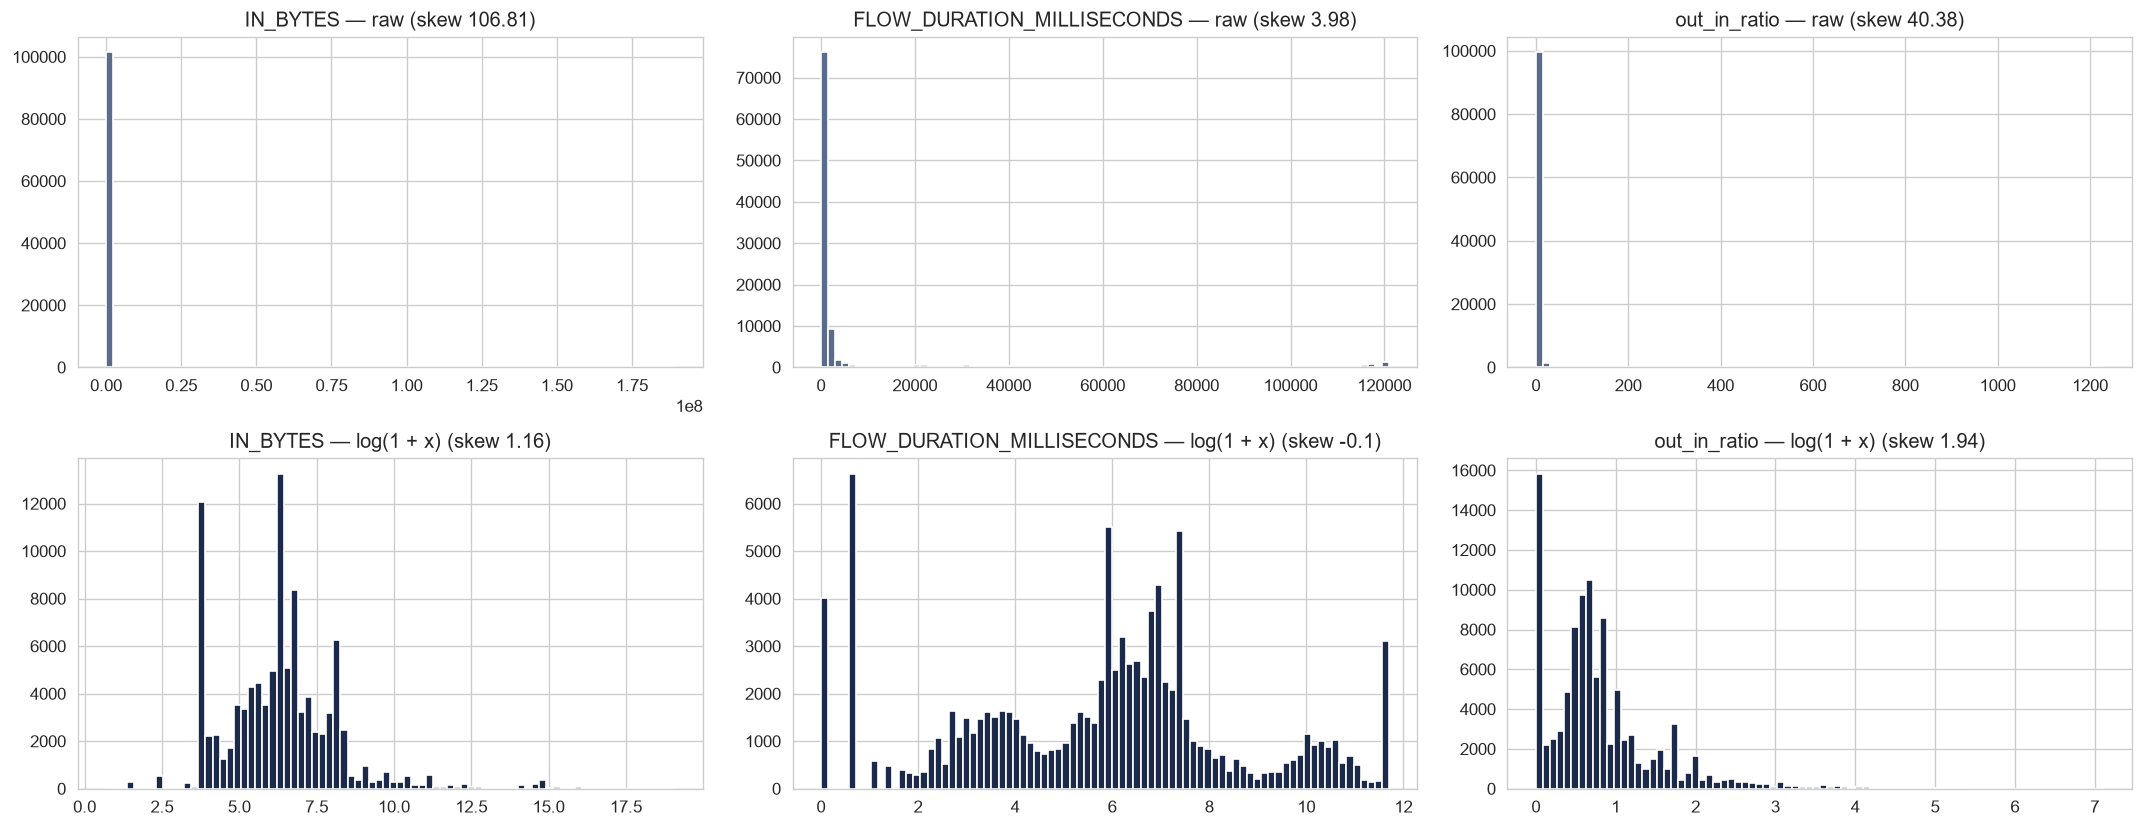
\includegraphics[width=\linewidth]{NetFlow_fe_log_before_after.png}
\caption{Three columns before (top) and after (bottom) $\log(1+x)$ (sample).}
\end{figure}

\begin{table}[H]\centering\small
\caption{Skewness before and after the log transformation (examples; sample).}
\begin{tabular}{lrr}
\toprule
Column & Before & After \\
\midrule
\var{IN_BYTES} & 106.8 & 1.16 \\
\var{OUT_BYTES} & 100.8 & $-0.41$ \\
\var{FLOW_DURATION_MILLISECONDS} & 3.98 & $-0.10$ \\
\var{LONGEST_FLOW_PKT} & 39.1 & $-0.08$ \\
\var{DNS_TTL_ANSWER} & 319.1 & 5.39 \\
\var{RETRANSMITTED_OUT_PKTS} & 60.9 & 3.56 \\
\var{pkts_per_sec} & 5.21 & 0.17 \\
\midrule
Columns with $|$skewness$| \leq 1$ & 0 of 36 & 17 of 36 \\
\bottomrule
\end{tabular}
\end{table}

\begin{reading}
Before the transformation, all 36 columns are highly skewed; on the raw scale almost every value sits in the first bar
of the histogram. After $\log(1+x)$, 17 columns have $|$skewness$| \leq 1$ (for example the duration: 3.98 to $-0.10$),
and the others are strongly reduced (\var{IN_BYTES}: 107 to 1.2). The columns that stay above 1 are those where
\textbf{most values are 0} (retransmissions, packet-size bins, minimum gaps). Their skewness comes from a spike at 0, not
from a long tail, and no transformation can spread a single value. The log still removes their extreme tail.
\end{reading}

\subsection{Robust scaling}

After the log, the columns still have different ranges. Each numeric column is scaled as
$(x - \text{median}) / \text{IQR}$, the same as scikit-learn's \texttt{RobustScaler}. The median and IQR are used instead
of the mean and standard deviation because \textbf{the outliers are the attacks}: with the mean and standard deviation, a
few extreme floods would set the scale for everything else. The 0/1 columns are left as they are.

\textbf{Special case, IQR = 0.} Five columns (the 4 retransmission columns and \var{DNS_TTL_ANSWER}) are 0 for more than
half of the behaviours, so their IQR is 0. They are divided by their \textbf{standard deviation} instead.

\begin{reading}
The special case was checked in practice. A first run left these five columns unscaled, as \texttt{RobustScaler} does.
Their spread (0 to 14) then dominated the PCA: the first component was made almost only of retransmissions. After the
fix, the scaled columns have a typical spread of about 1 (standard deviation 0.6 to 0.8 in the sample), so no column
dominates because of its unit.
\end{reading}

\section{Feature selection}

The 72 candidates (36 numeric, 4 created flags, 32 encoded) go through five steps; each removal has a reason.

\begin{enumerate}
  \item \textbf{Exact copies:} a column identical to another adds nothing.
  \item \textbf{Testbed fingerprints:} columns that identify the lab's machines rather than the attack (decision M10).
  \item \textbf{Near-constant columns:} one value in $\geq 99.5\%$ of all behaviours.
  \item \textbf{Highly correlated pairs:} $|$Spearman $\rho| \geq 0.95$ (the same rule as the CICIoT2023 part); the column
        with the lower mutual information with the family is removed.
  \item \textbf{Mutual information ranking} of the remaining features.
\end{enumerate}

\begin{table}[H]\centering\small
\caption{The 13 removed features.}
\begin{tabular}{lll}
\toprule
Feature & Step & Reason \\
\midrule
\var{TCP_WIN_MAX_IN}, \var{TCP_WIN_MAX_OUT} & fingerprint & window size set by each lab machine's OS (M10) \\
\var{client_urg} & near-constant & one value in 99.96\% of behaviours \\
\var{server_urg} & near-constant & one value in 100.00\% \\
\var{server_cwr} & near-constant & one value in 99.79\% \\
\var{client_ece} & correlated & $\rho = 1.00$ with \var{client_cwr} \\
\var{RETRANSMITTED_OUT_PKTS} & correlated & $\rho = 0.997$ with \var{RETRANSMITTED_OUT_BYTES} \\
\var{RETRANSMITTED_IN_PKTS} & correlated & $\rho = 0.984$ with \var{RETRANSMITTED_IN_BYTES} \\
\var{proto_tcp} & correlated & $\rho = -0.976$ with \var{proto_udp} \\
\var{l7_dns} & correlated & $\rho = 0.971$ with \var{DNS_TTL_ANSWER} \\
\var{DST_TO_SRC_IAT_AVG} & correlated & $\rho = 0.965$ with \var{DST_TO_SRC_IAT_MAX} \\
\var{SRC_TO_DST_IAT_AVG} & correlated & $\rho = 0.958$ with \var{SRC_TO_DST_IAT_MAX} \\
\var{bytes_per_sec} & correlated & $\rho = 0.950$ with \var{SRC_TO_DST_AVG_THROUGHPUT} \\
\bottomrule
\end{tabular}
\end{table}

\begin{reading}
Of the 72 candidates, \textbf{13 are removed} and \textbf{59 are kept}.
\begin{itemize}
  \item \textbf{No exact copies:} phase 3 had already dropped the copy columns (M7, M8).
  \item \textbf{2 fingerprints:} phase 4 showed that each family uses one TCP window size, set by the operating system
        of the lab machine. A model would learn the testbed, not the attack.
  \item \textbf{3 near-constant flags} carry almost no information.
  \item \textbf{8 correlated pairs:} retransmitted packets duplicate retransmitted bytes; \var{proto_tcp} is almost the
        opposite of \var{proto_udp}; \var{l7_dns} duplicates \var{DNS_TTL_ANSWER} (only DNS flows have an answer
        TTL); the average gap duplicates the largest gap; \var{bytes_per_sec} duplicates the existing throughput.
\end{itemize}
Only one of the 9 created features is removed (a near-copy of an existing column), so the other 8 add new information.
\end{reading}

\begin{figure}[H]\centering
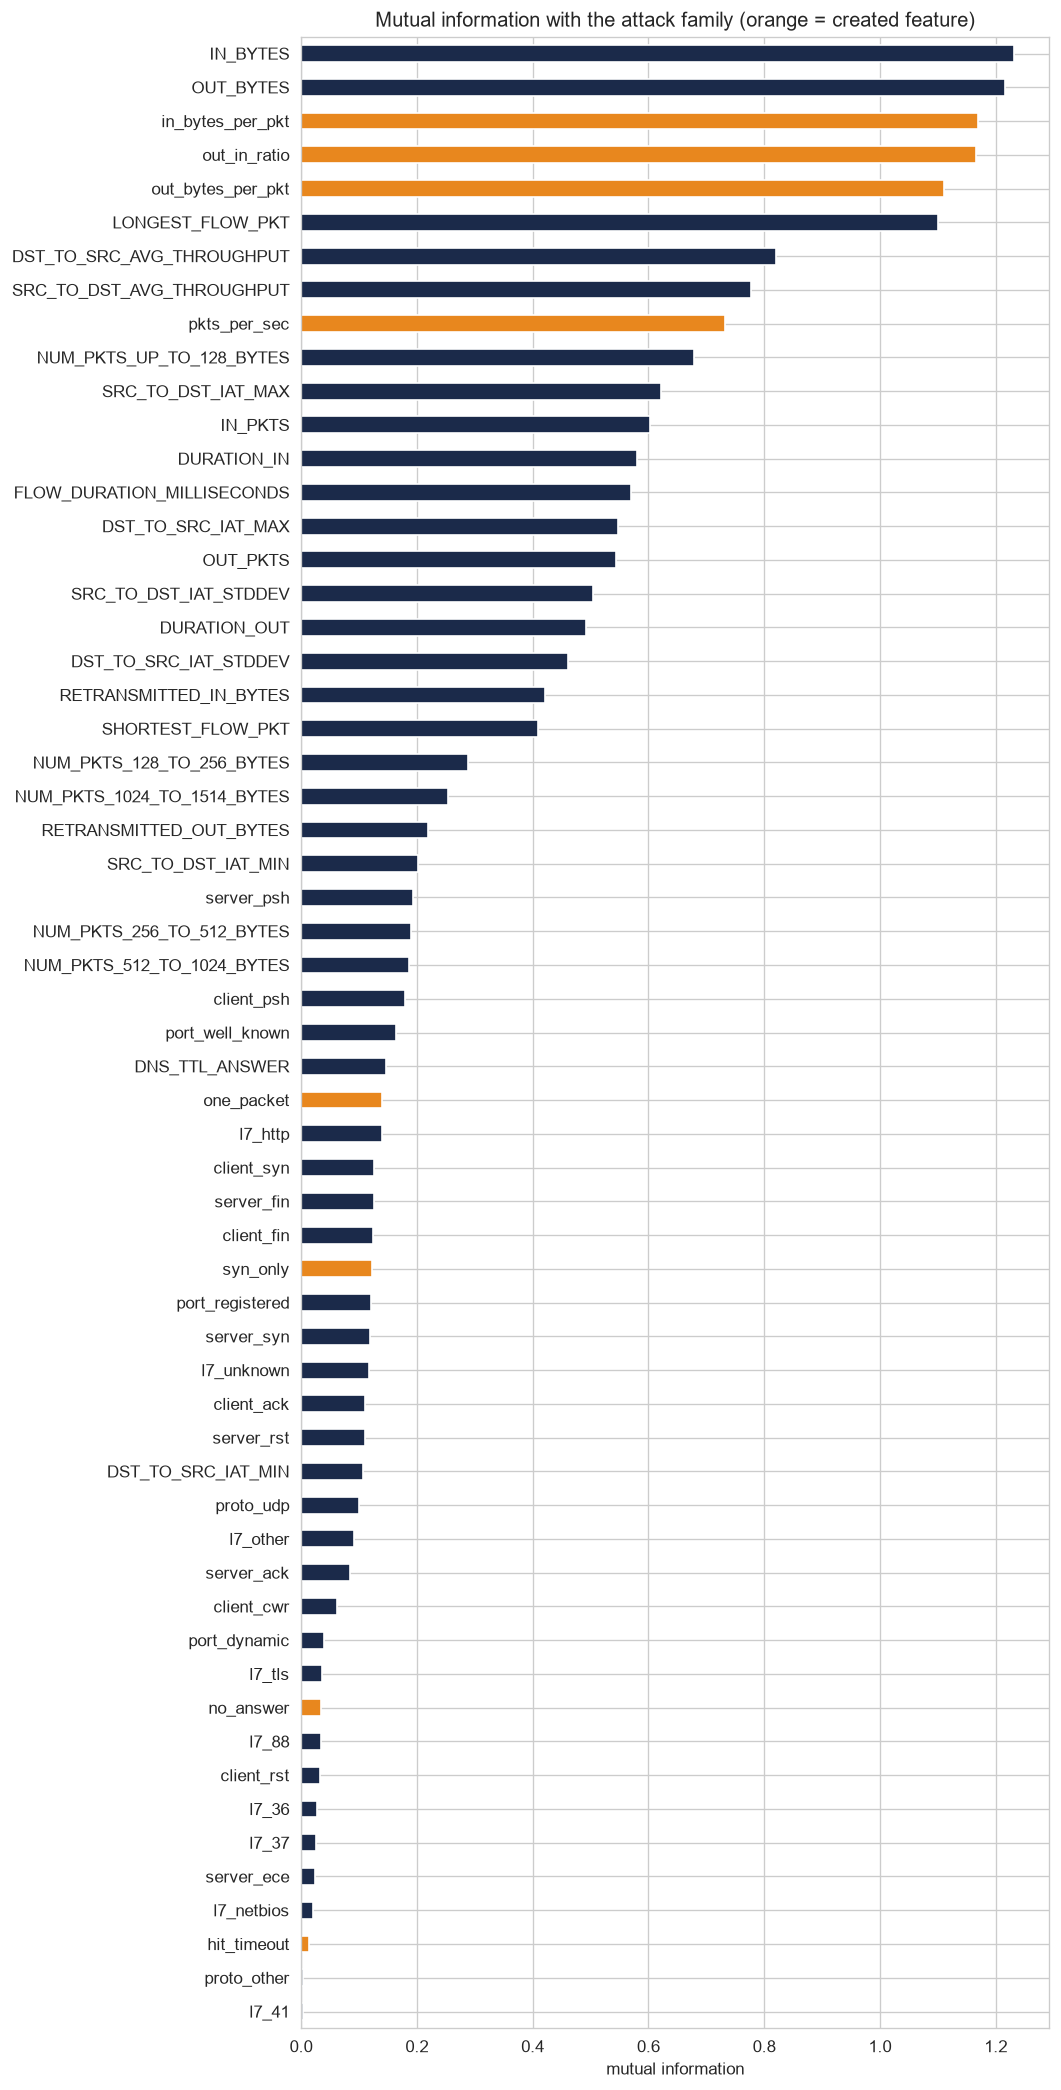
\includegraphics[height=0.62\textheight]{NetFlow_fe_mutual_information.png}
\caption{Mutual information of the 59 final features with the attack family (orange = created feature; sample).}
\end{figure}

\begin{reading}
The most informative features are the volume and packet-size features: \var{IN_BYTES} (1.23), \var{OUT_BYTES} (1.22),
then three \textbf{created} features, \var{in_bytes_per_pkt} (1.17), \var{out_in_ratio} (1.17) and
\var{out_bytes_per_pkt} (1.11). \textbf{Three of the top five are created features}, which justifies their creation.
The 0/1 columns score lower (at most 0.19). This is expected: a yes/no column can carry at most $\ln 2 \approx 0.69$ of
information. It does not make them useless (\var{syn_only} alone marks 92\% of the scans), so they are compared with each
other, not with the numeric columns.
\end{reading}

\clearpage
\section{Final feature set}

\subsection{From 53 raw columns to 59 features}

The four NetFlow v3 datasets share \textbf{53 traffic columns} (plus the two label columns). The table follows every
column from the raw files to the final feature set.

\begin{table}[H]\centering\small
\caption{How the number of columns changes, stage by stage.}
\begin{tabular}{L{4.3cm}rL{9.6cm}}
\toprule
Stage & Columns & What changes \\
\midrule
Raw NetFlow v3 files & 53 & the same 53 columns in UNSW, CIC-2018, ToN-IoT and BoT-IoT \\
Phases 2--3 (cleaning, merge) & 46 & $-2$ IP addresses (M3), $-2$ bytes-per-second columns with NaN / inf (U2, B2, C3, T3),
  $-2$ IP packet-length copies (M7), $-1$ \var{TCP_FLAGS} and $-1$ \var{ICMP_IPV4_TYPE} copies (M8);
  $+1$ because \var{L7_PROTO} is split into \var{L7_MAIN} and \var{L7_SUB} (U3) \\
Phase 5, step 0 (never features) & 39 & $-7$: 2 timestamps (M2), source port and DNS query ID (M5), 2 TTL (M4), FTP
  return code (M10). Left: \textbf{31 numeric} and \textbf{8 code} columns \\
Phase 5, encoding & 63 & the 8 code columns become \textbf{32} yes/no columns; \var{L7_SUB}, \var{ICMP_TYPE} and
  \var{DNS_QUERY_TYPE} are not encoded (too rare or already covered) \\
Phase 5, creation & 72 & $+9$ created features (5 ratios and rates, 4 behaviour flags): the \textbf{72 candidates} \\
Phase 5, selection & \textbf{59} & $-13$: 2 fingerprints, 3 near-constant, 8 correlated (section 6) \\
\bottomrule
\end{tabular}
\end{table}

\begin{table}[H]\centering\small
\caption{Candidates, removed and kept, per group.}
\begin{tabular}{L{3.2cm}rrrL{7.0cm}}
\toprule
Group & Candidates & Removed & Kept & Removed columns \\
\midrule
Original numeric & 31 & 6 & \textbf{25} & \var{TCP_WIN_MAX_IN}, \var{TCP_WIN_MAX_OUT} (fingerprints);
  \var{RETRANSMITTED_IN_PKTS}, \var{RETRANSMITTED_OUT_PKTS}, \var{SRC_TO_DST_IAT_AVG}, \var{DST_TO_SRC_IAT_AVG} (correlated) \\
Created & 9 & 1 & \textbf{8} & \var{bytes_per_sec} (correlated with the existing throughput) \\
Encoded & 32 & 6 & \textbf{26} & \var{client_urg}, \var{server_urg}, \var{server_cwr} (near-constant);
  \var{client_ece}, \var{proto_tcp}, \var{l7_dns} (correlated) \\
\midrule
\textbf{Total} & \textbf{72} & \textbf{13} & \textbf{59} & \\
\bottomrule
\end{tabular}
\end{table}

\begin{table}[H]\centering\small
\caption{The 59 final features by what they describe.}
\begin{tabular}{L{3.1cm}rL{11.1cm}}
\toprule
What it describes & Count & Features \\
\midrule
Volume & 6 & \var{IN_BYTES}, \var{OUT_BYTES}, \var{IN_PKTS}, \var{OUT_PKTS}, \var{RETRANSMITTED_IN_BYTES},
  \var{RETRANSMITTED_OUT_BYTES} \\
Packet sizes & 7 & \var{LONGEST_FLOW_PKT}, \var{SHORTEST_FLOW_PKT}, and the 5 size bins \var{NUM_PKTS_UP_TO_128_BYTES}
  \ldots\ \var{NUM_PKTS_1024_TO_1514_BYTES} \\
Time and rate & 11 & \var{FLOW_DURATION_MILLISECONDS}, \var{DURATION_IN}, \var{DURATION_OUT}, the 2 average throughputs,
  and the minimum, maximum and standard deviation of the gaps between packets in each direction (6) \\
DNS & 1 & \var{DNS_TTL_ANSWER} \\
\midrule
\multicolumn{3}{l}{\emph{Original numeric columns: 25}} \\
\midrule
Created: ratios and rates & 4 & \var{in_bytes_per_pkt}, \var{out_bytes_per_pkt}, \var{out_in_ratio}, \var{pkts_per_sec} \\
Created: behaviour flags & 4 & \var{no_answer}, \var{one_packet}, \var{syn_only}, \var{hit_timeout} \\
\midrule
\multicolumn{3}{l}{\emph{Created features: 8}} \\
\midrule
Destination port range & 3 & \var{port_well_known}, \var{port_registered}, \var{port_dynamic} \\
Protocol & 2 & \var{proto_udp}, \var{proto_other} (TCP = both 0) \\
Client TCP flags & 6 & \var{client_fin}, \var{client_syn}, \var{client_rst}, \var{client_psh}, \var{client_ack},
  \var{client_cwr} \\
Server TCP flags & 6 & \var{server_fin}, \var{server_syn}, \var{server_rst}, \var{server_psh}, \var{server_ack},
  \var{server_ece} \\
Application protocol & 9 & \var{l7_http}, \var{l7_tls}, \var{l7_unknown}, \var{l7_netbios}, \var{l7_88}, \var{l7_36},
  \var{l7_37}, \var{l7_41}, \var{l7_other} (DNS flows are recognised by \var{DNS_TTL_ANSWER}) \\
\midrule
\multicolumn{3}{l}{\emph{Encoded columns: 26}} \\
\midrule
\textbf{Total} & \textbf{59} & \\
\bottomrule
\end{tabular}
\end{table}

\begin{reading}
\begin{itemize}
  \item \textbf{Most features are original NetFlow measurements} (25 of 59). Only 6 of the 31 numeric traffic columns
        were removed: 2 because they identify the lab's machines, 4 because they repeated another column.
  \item \textbf{8 of the 9 created features are kept;} the only one removed, \var{bytes_per_sec}, duplicated an
        existing throughput column.
  \item \textbf{The 26 encoded columns turn 5 code columns into usable yes/no information:}
        \begin{itemize}
          \item port range, protocol and application protocol: the type of service;
          \item 12 TCP flags: how the connection behaved.
        \end{itemize}
  \item \textbf{Two encoded groups lost one column with no loss of information:}
        \begin{itemize}
          \item \var{proto_tcp} is implied when \var{proto_udp} and \var{proto_other} are both 0;
          \item \var{l7_dns} is carried by \var{DNS_TTL_ANSWER}.
        \end{itemize}
\end{itemize}
\end{reading}

\subsection{Justification of the final set}

\begin{reading}
The final set has \textbf{59 features}: 25 original numeric columns, 8 created features and 26 encoded columns.
\begin{itemize}
  \item \textbf{Based on evidence:} every feature comes from a phase 2 decision or a phase 4 finding.
  \item \textbf{No identifier of the network or the moment:} no IP address, timestamp or TTL, and the TCP window is
        removed as a fingerprint.
  \item \textbf{No duplicates:} no pair has $|\rho| \geq 0.95$.
  \item \textbf{No useless columns:} no column is near-constant.
  \item \textbf{Ready for a model:} every numeric column is log-transformed and robust-scaled, and every code is one-hot
        encoded.
\end{itemize}
The final dataset keeps all 17,551,848 behaviours with the 59 features and 6 label/weight columns (634\,MB):
\begin{itemize}
  \item data: \texttt{data/processed/netflow\_features.parquet};
  \item data dictionary: \texttt{tables/NetFlow\_fe\_dictionary.csv}.
\end{itemize}
\end{reading}

{\small
\begin{longtable}{p{5.2cm}p{6.6cm}lr}
\caption{The 59 final features, ordered by mutual information (MI) with the family. Numeric features are
log-transformed and robust-scaled; 0/1 features are not transformed.}\\
\toprule
Feature & Meaning & Origin & MI \\
\midrule
\endfirsthead
\toprule
Feature & Meaning & Origin & MI \\
\midrule
\endhead
\bottomrule
\endfoot
\var{IN_BYTES} & bytes sent by the client & original & 1.231 \\
\var{OUT_BYTES} & bytes sent back by the server & original & 1.216 \\
\var{in_bytes_per_pkt} & average size of the packets sent & created & 1.169 \\
\var{out_in_ratio} & bytes received per byte sent & created & 1.165 \\
\var{out_bytes_per_pkt} & average size of the packets received & created & 1.110 \\
\var{LONGEST_FLOW_PKT} & largest packet of the flow & original & 1.100 \\
\var{DST_TO_SRC_AVG_THROUGHPUT} & average throughput server to client & original & 0.820 \\
\var{SRC_TO_DST_AVG_THROUGHPUT} & average throughput client to server & original & 0.778 \\
\var{pkts_per_sec} & packets per second (both directions) & created & 0.733 \\
\var{NUM_PKTS_UP_TO_128_BYTES} & packets of at most 128 bytes & original & 0.679 \\
\var{SRC_TO_DST_IAT_MAX} & largest gap between client packets & original & 0.622 \\
\var{IN_PKTS} & packets sent by the client & original & 0.602 \\
\var{DURATION_IN} & duration of the client-to-server stream & original & 0.579 \\
\var{FLOW_DURATION_MILLISECONDS} & duration of the flow & original & 0.570 \\
\var{DST_TO_SRC_IAT_MAX} & largest gap between server packets & original & 0.547 \\
\var{OUT_PKTS} & packets sent back by the server & original & 0.544 \\
\var{SRC_TO_DST_IAT_STDDEV} & spread of the gaps between client packets & original & 0.505 \\
\var{DURATION_OUT} & duration of the server-to-client stream & original & 0.492 \\
\var{DST_TO_SRC_IAT_STDDEV} & spread of the gaps between server packets & original & 0.462 \\
\var{RETRANSMITTED_IN_BYTES} & bytes retransmitted by the client & original & 0.420 \\
\var{SHORTEST_FLOW_PKT} & smallest packet of the flow & original & 0.409 \\
\var{NUM_PKTS_128_TO_256_BYTES} & packets of 128--256 bytes & original & 0.288 \\
\var{NUM_PKTS_1024_TO_1514_BYTES} & packets of 1024--1514 bytes & original & 0.254 \\
\var{RETRANSMITTED_OUT_BYTES} & bytes retransmitted by the server & original & 0.219 \\
\var{SRC_TO_DST_IAT_MIN} & smallest gap between client packets & original & 0.202 \\
\var{server_psh} & 1 if the server set the PSH flag & encoded & 0.193 \\
\var{NUM_PKTS_256_TO_512_BYTES} & packets of 256--512 bytes & original & 0.190 \\
\var{NUM_PKTS_512_TO_1024_BYTES} & packets of 512--1024 bytes & original & 0.186 \\
\var{client_psh} & 1 if the client set the PSH flag & encoded & 0.180 \\
\var{port_well_known} & 1 if the destination port is 0--1023 & encoded & 0.164 \\
\var{DNS_TTL_ANSWER} & time-to-live of the DNS answer & original & 0.146 \\
\var{one_packet} & 1 if the client sent a single packet & created & 0.140 \\
\var{l7_http} & 1 if the application protocol is HTTP & encoded & 0.139 \\
\var{client_syn} & 1 if the client set the SYN flag & encoded & 0.126 \\
\var{server_fin} & 1 if the server set the FIN flag & encoded & 0.125 \\
\var{client_fin} & 1 if the client set the FIN flag & encoded & 0.124 \\
\var{syn_only} & 1 if TCP and the client sent only SYN (half-open scan) & created & 0.123 \\
\var{port_registered} & 1 if the destination port is 1024--49151 & encoded & 0.120 \\
\var{server_syn} & 1 if the server set the SYN flag & encoded & 0.119 \\
\var{l7_unknown} & 1 if the application protocol is unknown & encoded & 0.118 \\
\var{client_ack} & 1 if the client set the ACK flag & encoded & 0.111 \\
\var{server_rst} & 1 if the server set the RST flag & encoded & 0.111 \\
\var{DST_TO_SRC_IAT_MIN} & smallest gap between server packets & original & 0.106 \\
\var{proto_udp} & 1 if UDP & encoded & 0.100 \\
\var{l7_other} & 1 if a rare application protocol & encoded & 0.091 \\
\var{server_ack} & 1 if the server set the ACK flag & encoded & 0.084 \\
\var{client_cwr} & 1 if the client set the CWR flag & encoded & 0.062 \\
\var{port_dynamic} & 1 if the destination port is 49152 or more & encoded & 0.039 \\
\var{l7_tls} & 1 if the application protocol is TLS & encoded & 0.037 \\
\var{no_answer} & 1 if the server sent nothing back & created & 0.035 \\
\var{l7_88} & 1 if the application protocol is nDPI code 88 & encoded & 0.034 \\
\var{client_rst} & 1 if the client set the RST flag & encoded & 0.033 \\
\var{l7_36} & 1 if the application protocol is nDPI code 36 & encoded & 0.028 \\
\var{l7_37} & 1 if the application protocol is nDPI code 37 & encoded & 0.026 \\
\var{server_ece} & 1 if the server set the ECE flag & encoded & 0.025 \\
\var{l7_netbios} & 1 if the application protocol is NetBIOS & encoded & 0.020 \\
\var{hit_timeout} & 1 if the flow lasted 120\,s or more & created & 0.014 \\
\var{proto_other} & 1 if another protocol (ICMP, \ldots) & encoded & 0.004 \\
\var{l7_41} & 1 if the application protocol is nDPI code 41 & encoded & 0.003 \\
\end{longtable}
}

\section{PCA: a 2-D view of the families}

Principal component analysis builds new axes (components) as combinations of the features, ordered by how much of the
variation they explain. Two components give a map of the data: if the families form separate clouds, the features
separate them well. PCA is fitted on the sample with the 59 final features.

\begin{figure}[H]\centering
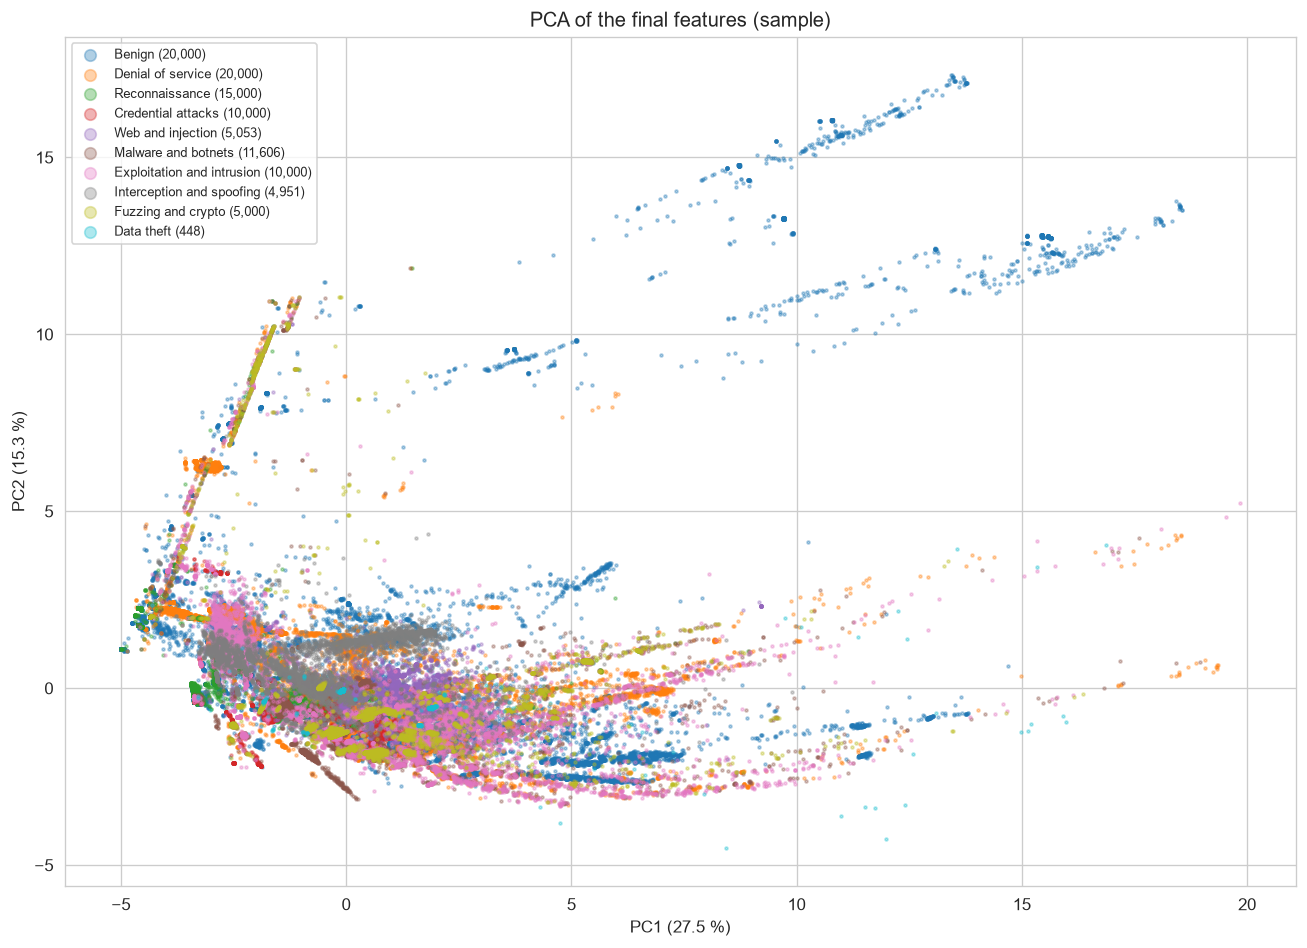
\includegraphics[width=0.85\linewidth]{NetFlow_fe_pca.png}
\caption{The sample projected on the first two principal components, coloured by family.}
\end{figure}

\begin{reading}
\begin{itemize}
  \item \textbf{Variance:} the first two components explain \textbf{42.8\%} of the variation, and 10 components explain
        85.8\%, so the 59 features do not reduce to two dimensions.
  \item \textbf{The two axes:} PC1 is the \textbf{size of the flow} (number of packets and packets of each size). PC2
        contrasts the smallest packet with the answer size and throughput.
  \item \textbf{Separate clusters:} Reconnaissance is a tight group on the left (tiny one-packet probes), and Fuzzing
        lies along its own line.
  \item \textbf{Benign} spreads over the whole map: normal traffic is the most varied.
  \item \textbf{Most attack families overlap} in the centre.
\end{itemize}
As in phase 4, no single direction separates the families: a model will need many features together. PCA is used here
to look at the data; the features themselves are kept for interpretability.
\end{reading}

\section{Techniques not used, and why}

\begin{table}[H]\centering\small
\begin{tabular}{L{4.2cm}L{1.6cm}L{9.4cm}}
\toprule
Technique & Used? & Why \\
\midrule
Date / hour-of-day features & no & timestamps reveal the lab's attack schedule (M2); a model would learn \emph{when} the lab ran each attack \\
Polynomial / interaction terms & no & the relationships found in phase 4 are monotonic, not curved; squared terms of about 60 columns would add about 1,800 columns without a reason \\
Binning of bytes, packets or durations & only the port & the log transform keeps the full detail; bins would throw it away. The port is binned because its number has no meaning, only its range \\
Target encoding & no & it builds a feature from the label (risk of leakage); no column has so many categories that one-hot is impossible \\
Train/test split, model-based importance & no & the project stops before modelling; mutual information ranks the features without a model \\
\bottomrule
\end{tabular}
\end{table}

\section{Conclusion}

\begin{enumerate}
  \item \textbf{The created features earn their place:} 8 of the 9 survive the selection, and 3 are among the 5 most
        informative features. Ratios and behaviour flags (one packet, SYN only, no answer) capture scans, floods and
        conversations directly.
  \item \textbf{Log transformation and robust scaling are necessary:} the data are extremely skewed, and the outliers are
        the attacks themselves. The special case IQR = 0 had to be handled so that no column dominates.
  \item \textbf{The final set keeps only traffic behaviour:} 59 features, with no column that identifies the network, the
        machine or the moment. This matters for SQ3, because a model must not recognise the lab instead of the attack.
\end{enumerate}
\textbf{Before modelling} (outside this project): split the data first, then refit the scaling and the selection on the
training part only.

\end{document}
